
% Service-specific notifications
\begin{figure}[ht]
    \resizebox{1\textwidth}{!}{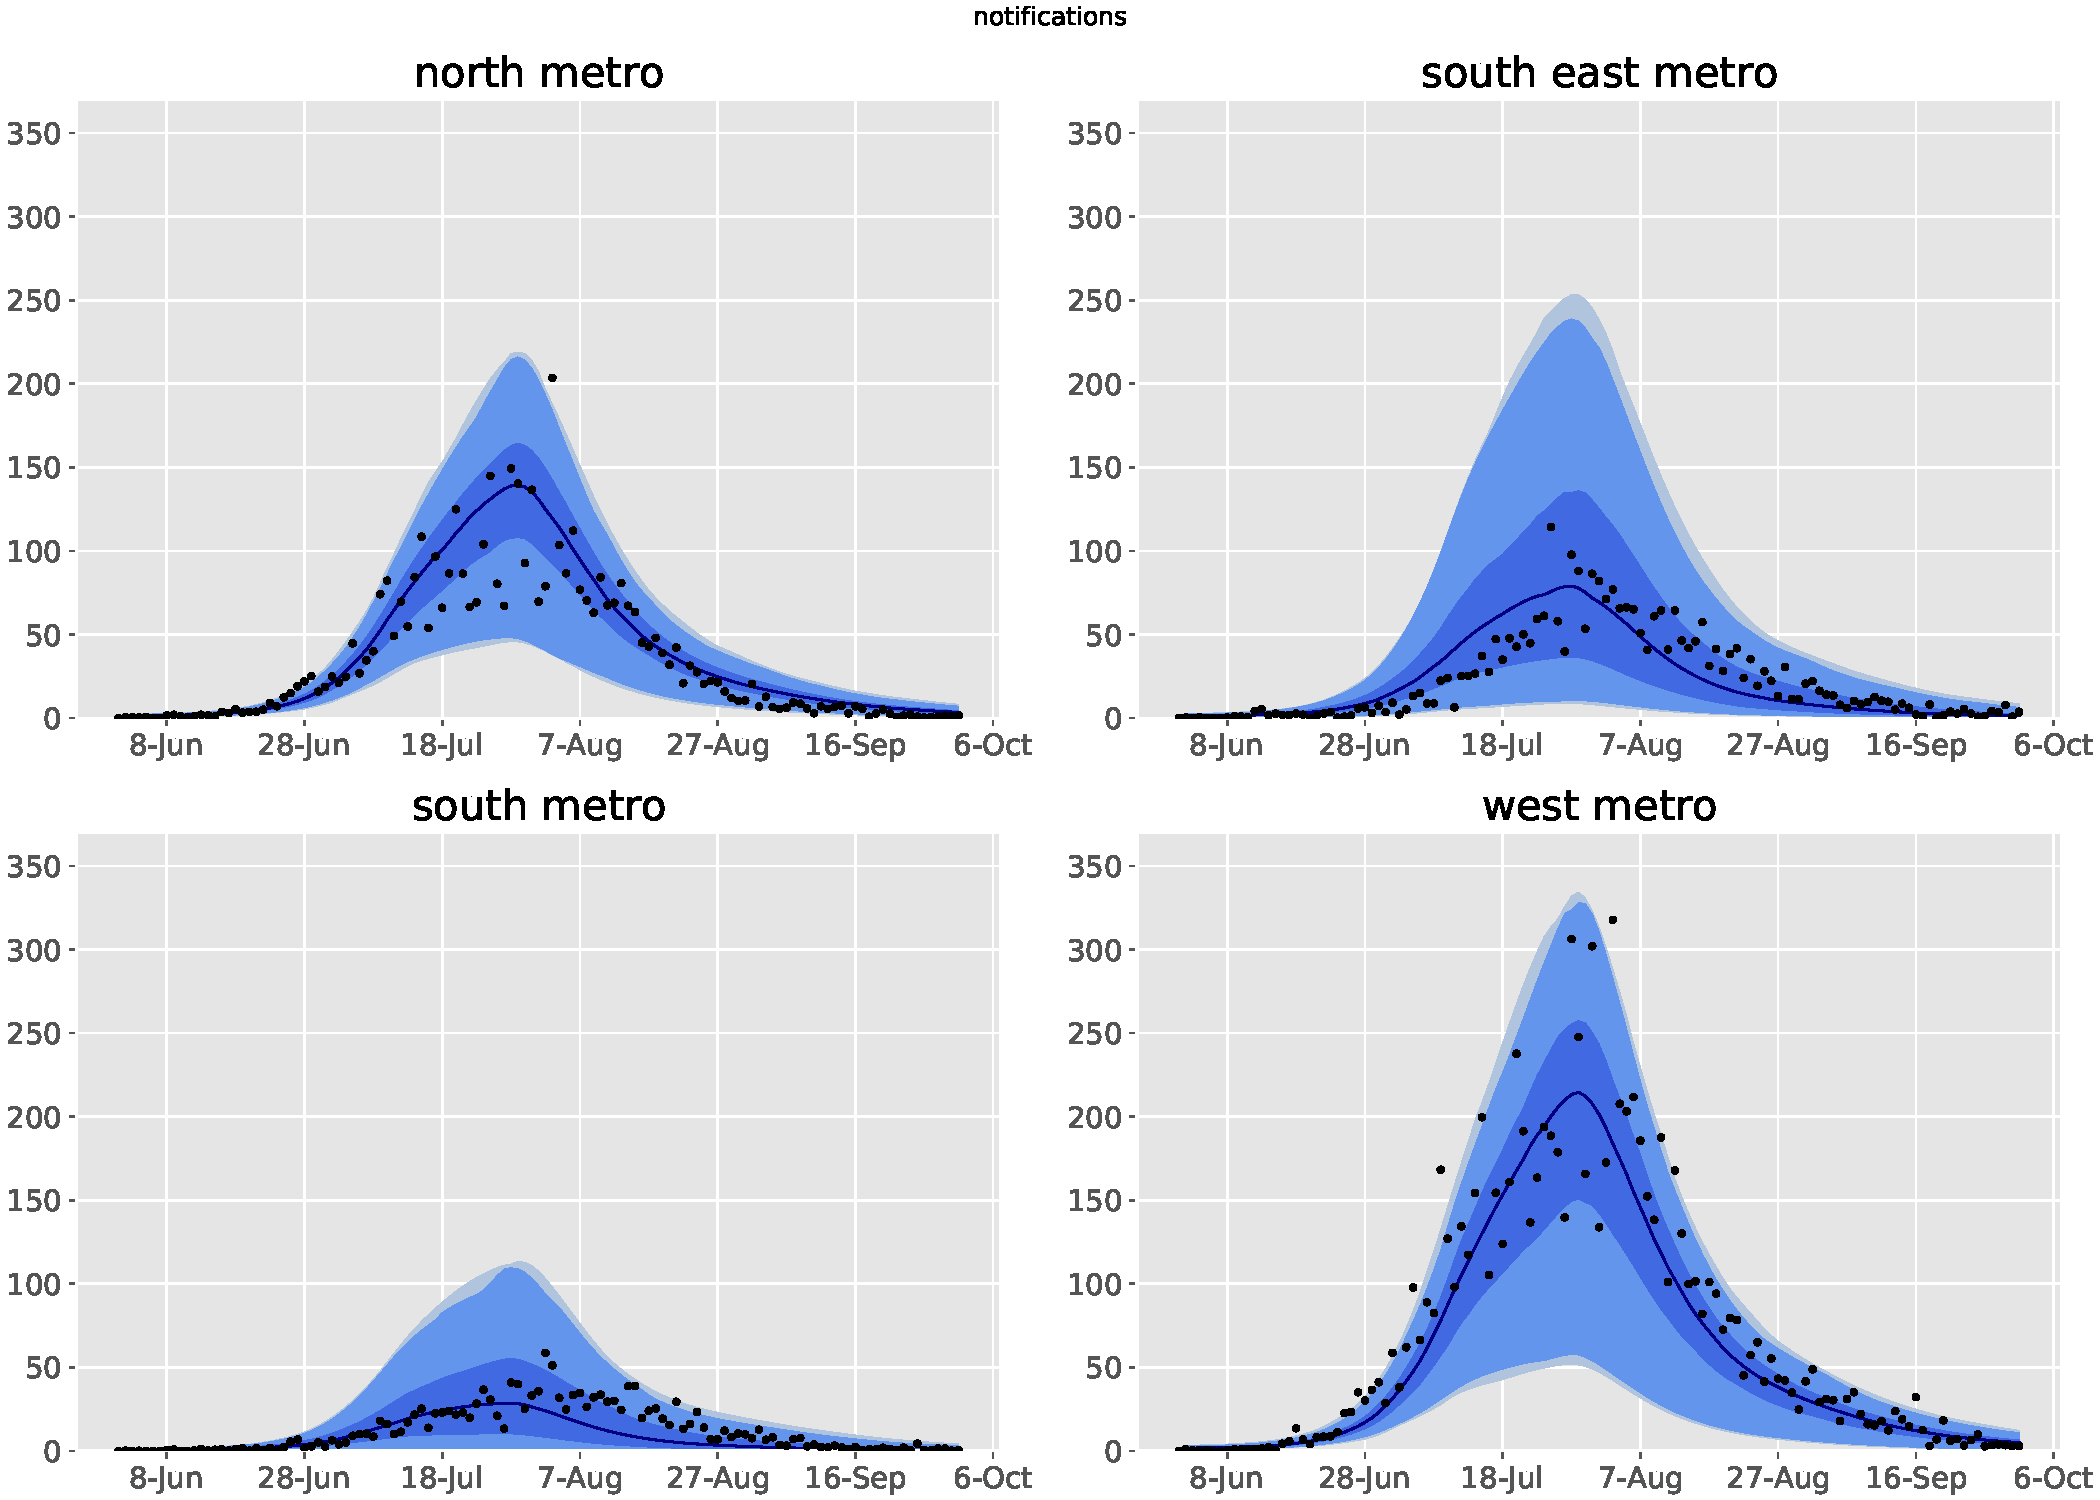
\includegraphics[scale=1]{../covid_19/projects/victoria/results_figures/metro_notifications.png}}
    \caption{\textbf{Calibration fit to daily time series of notifications for each metropolitan health service cluster.} Daily confirmed cases (black dots) overlaid on the median modelled detected cases (dark blue line), with shaded areas representing the 25\textsuperscript{th} to 75\textsuperscript{th} centile (mid blue), 2.5\textsuperscript{th} to 97.5\textsuperscript{th} centile (light blue) and 1\textsuperscript{st} to 99\textsuperscript{th} centile (faintest blue) of estimated detected cases.}
\end{figure}

\begin{figure}[ht]
    \resizebox{1\textwidth}{!}{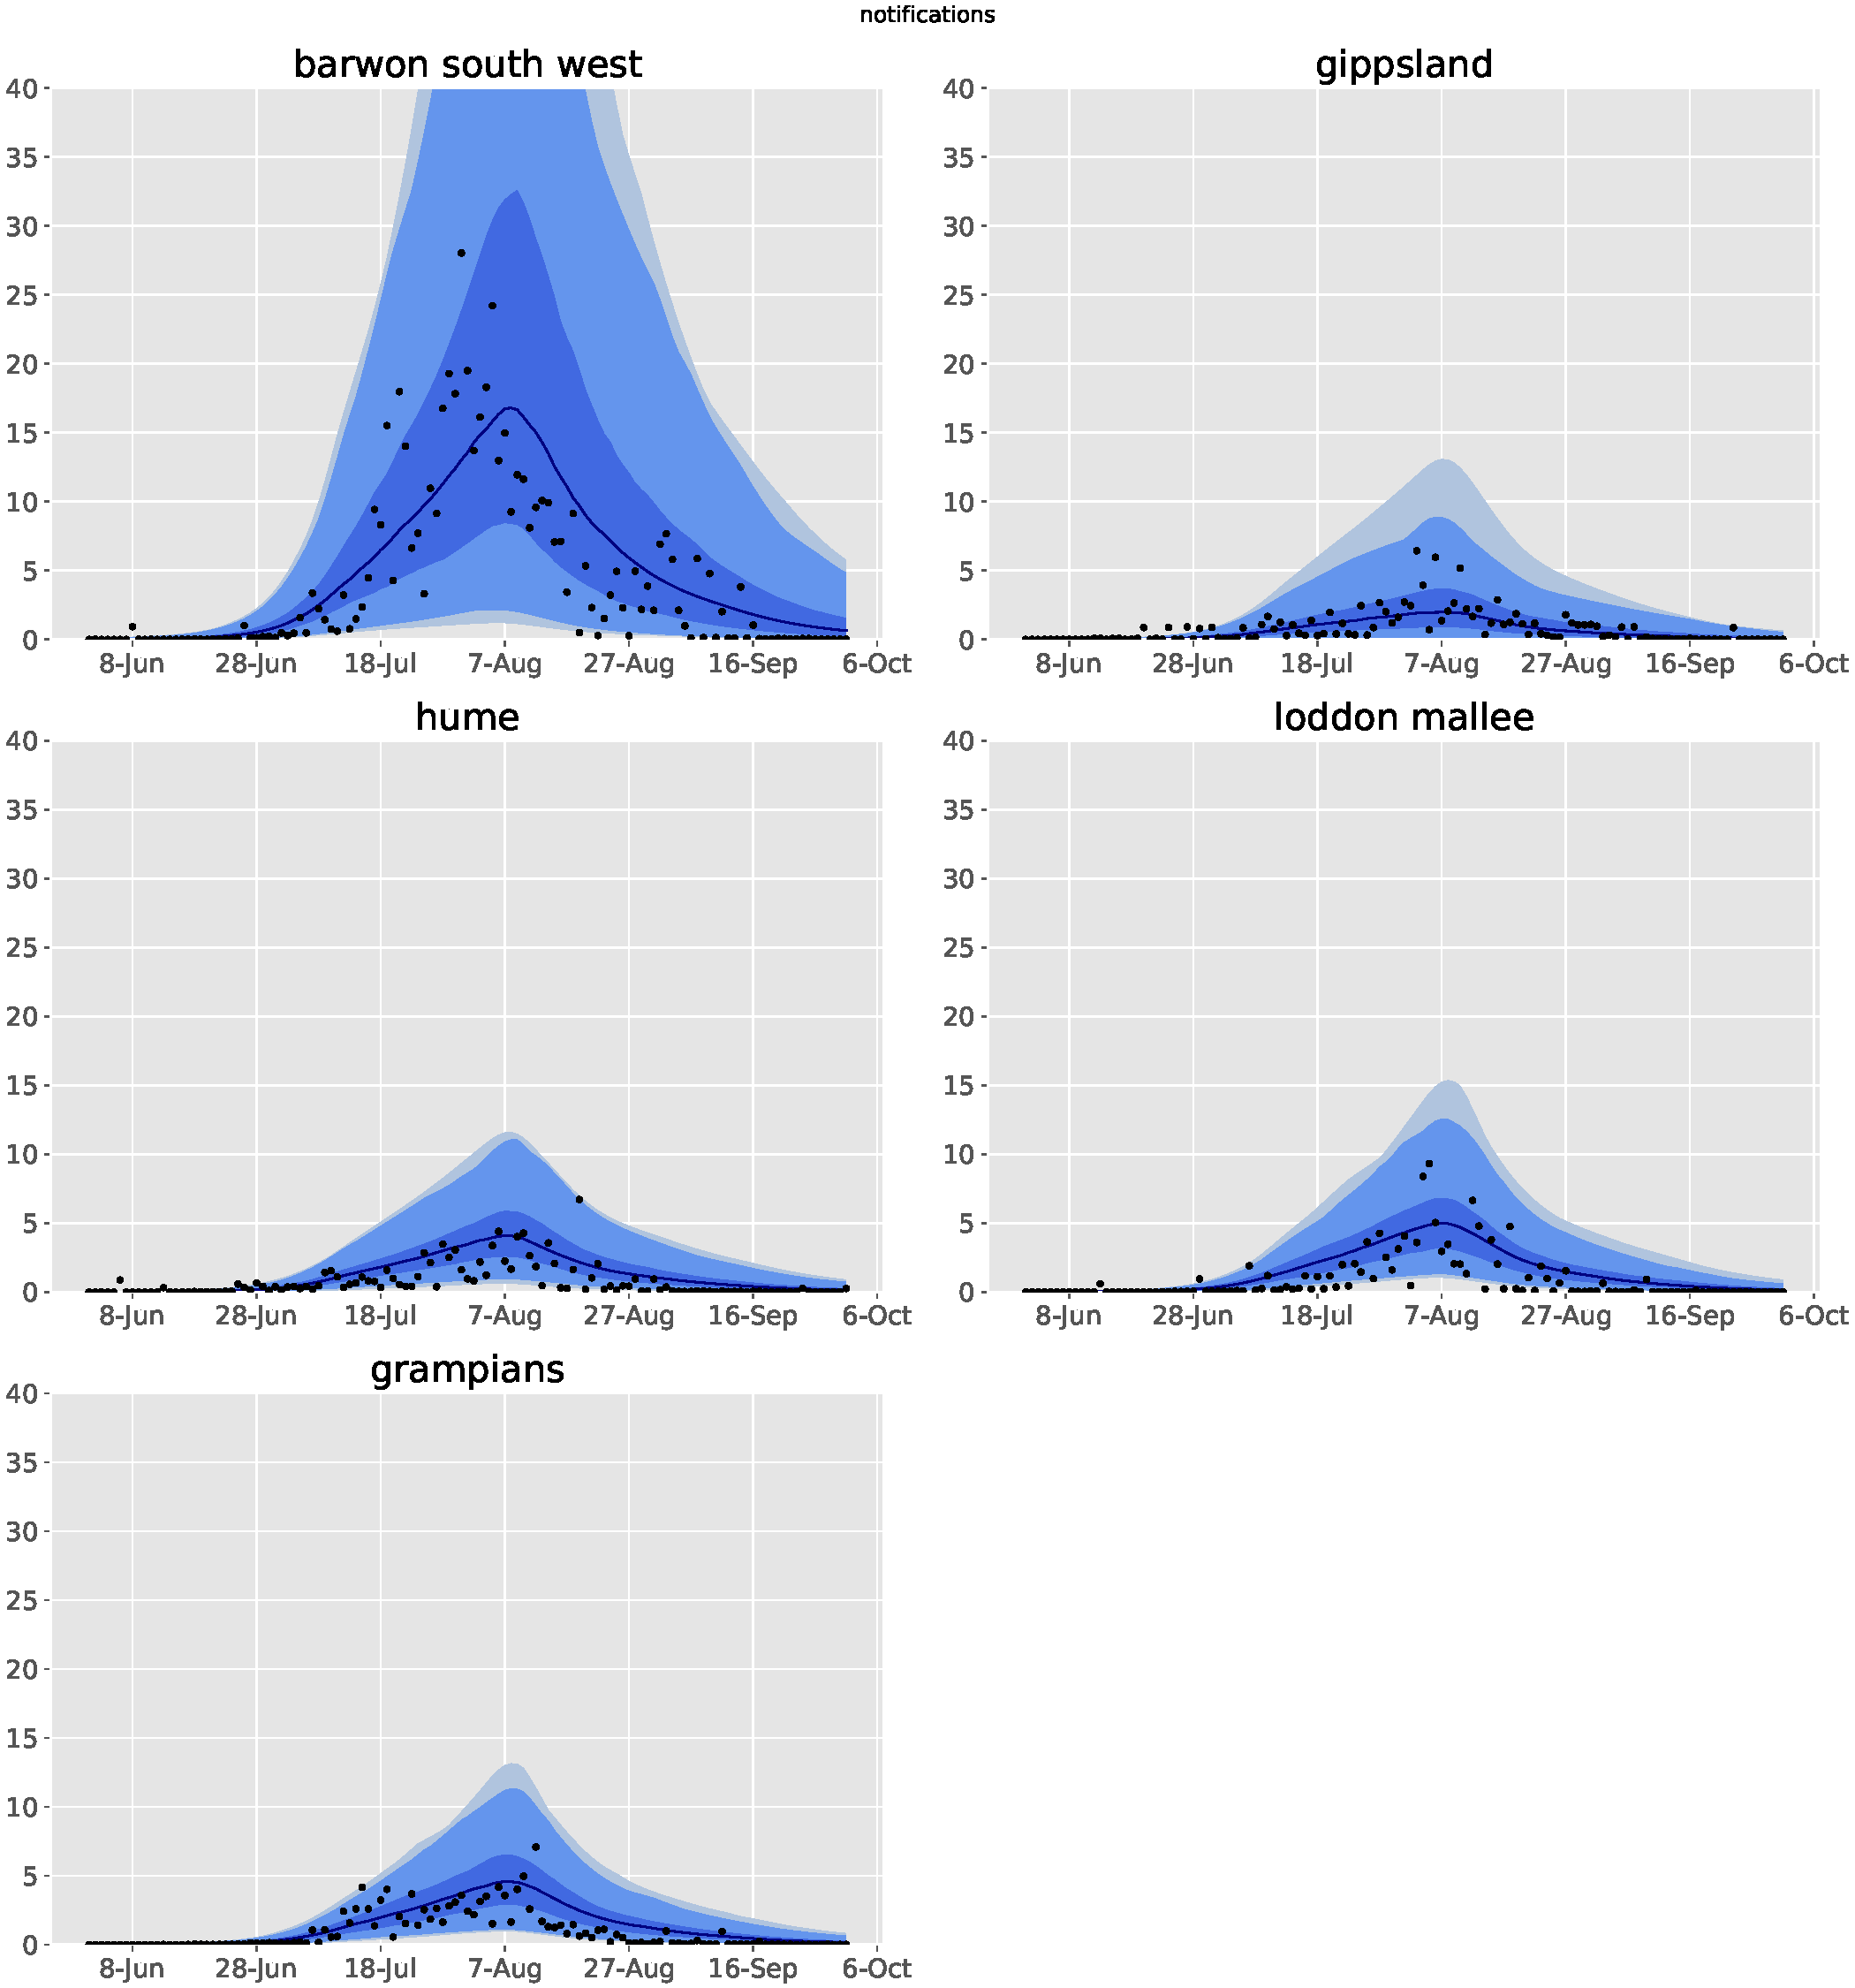
\includegraphics[scale=1]{../covid_19/projects/victoria/results_figures/regional_notifications.png}}
    \caption{\textbf{Calibration fit to daily time series of notifications for each regional health service cluster.} Daily confirmed cases (black dots) overlaid on the median modelled detected cases (dark blue line), with shaded areas representing the 25\textsuperscript{th} to 75\textsuperscript{th} centile (mid blue), 2.5\textsuperscript{th} to 97.5\textsuperscript{th} centile (light blue) and 1\textsuperscript{st} to 99\textsuperscript{th} centile (faintest blue) of estimated detected cases.}
\end{figure}

% Hospitalisations
\begin{figure}[ht]
    \resizebox{1\textwidth}{!}{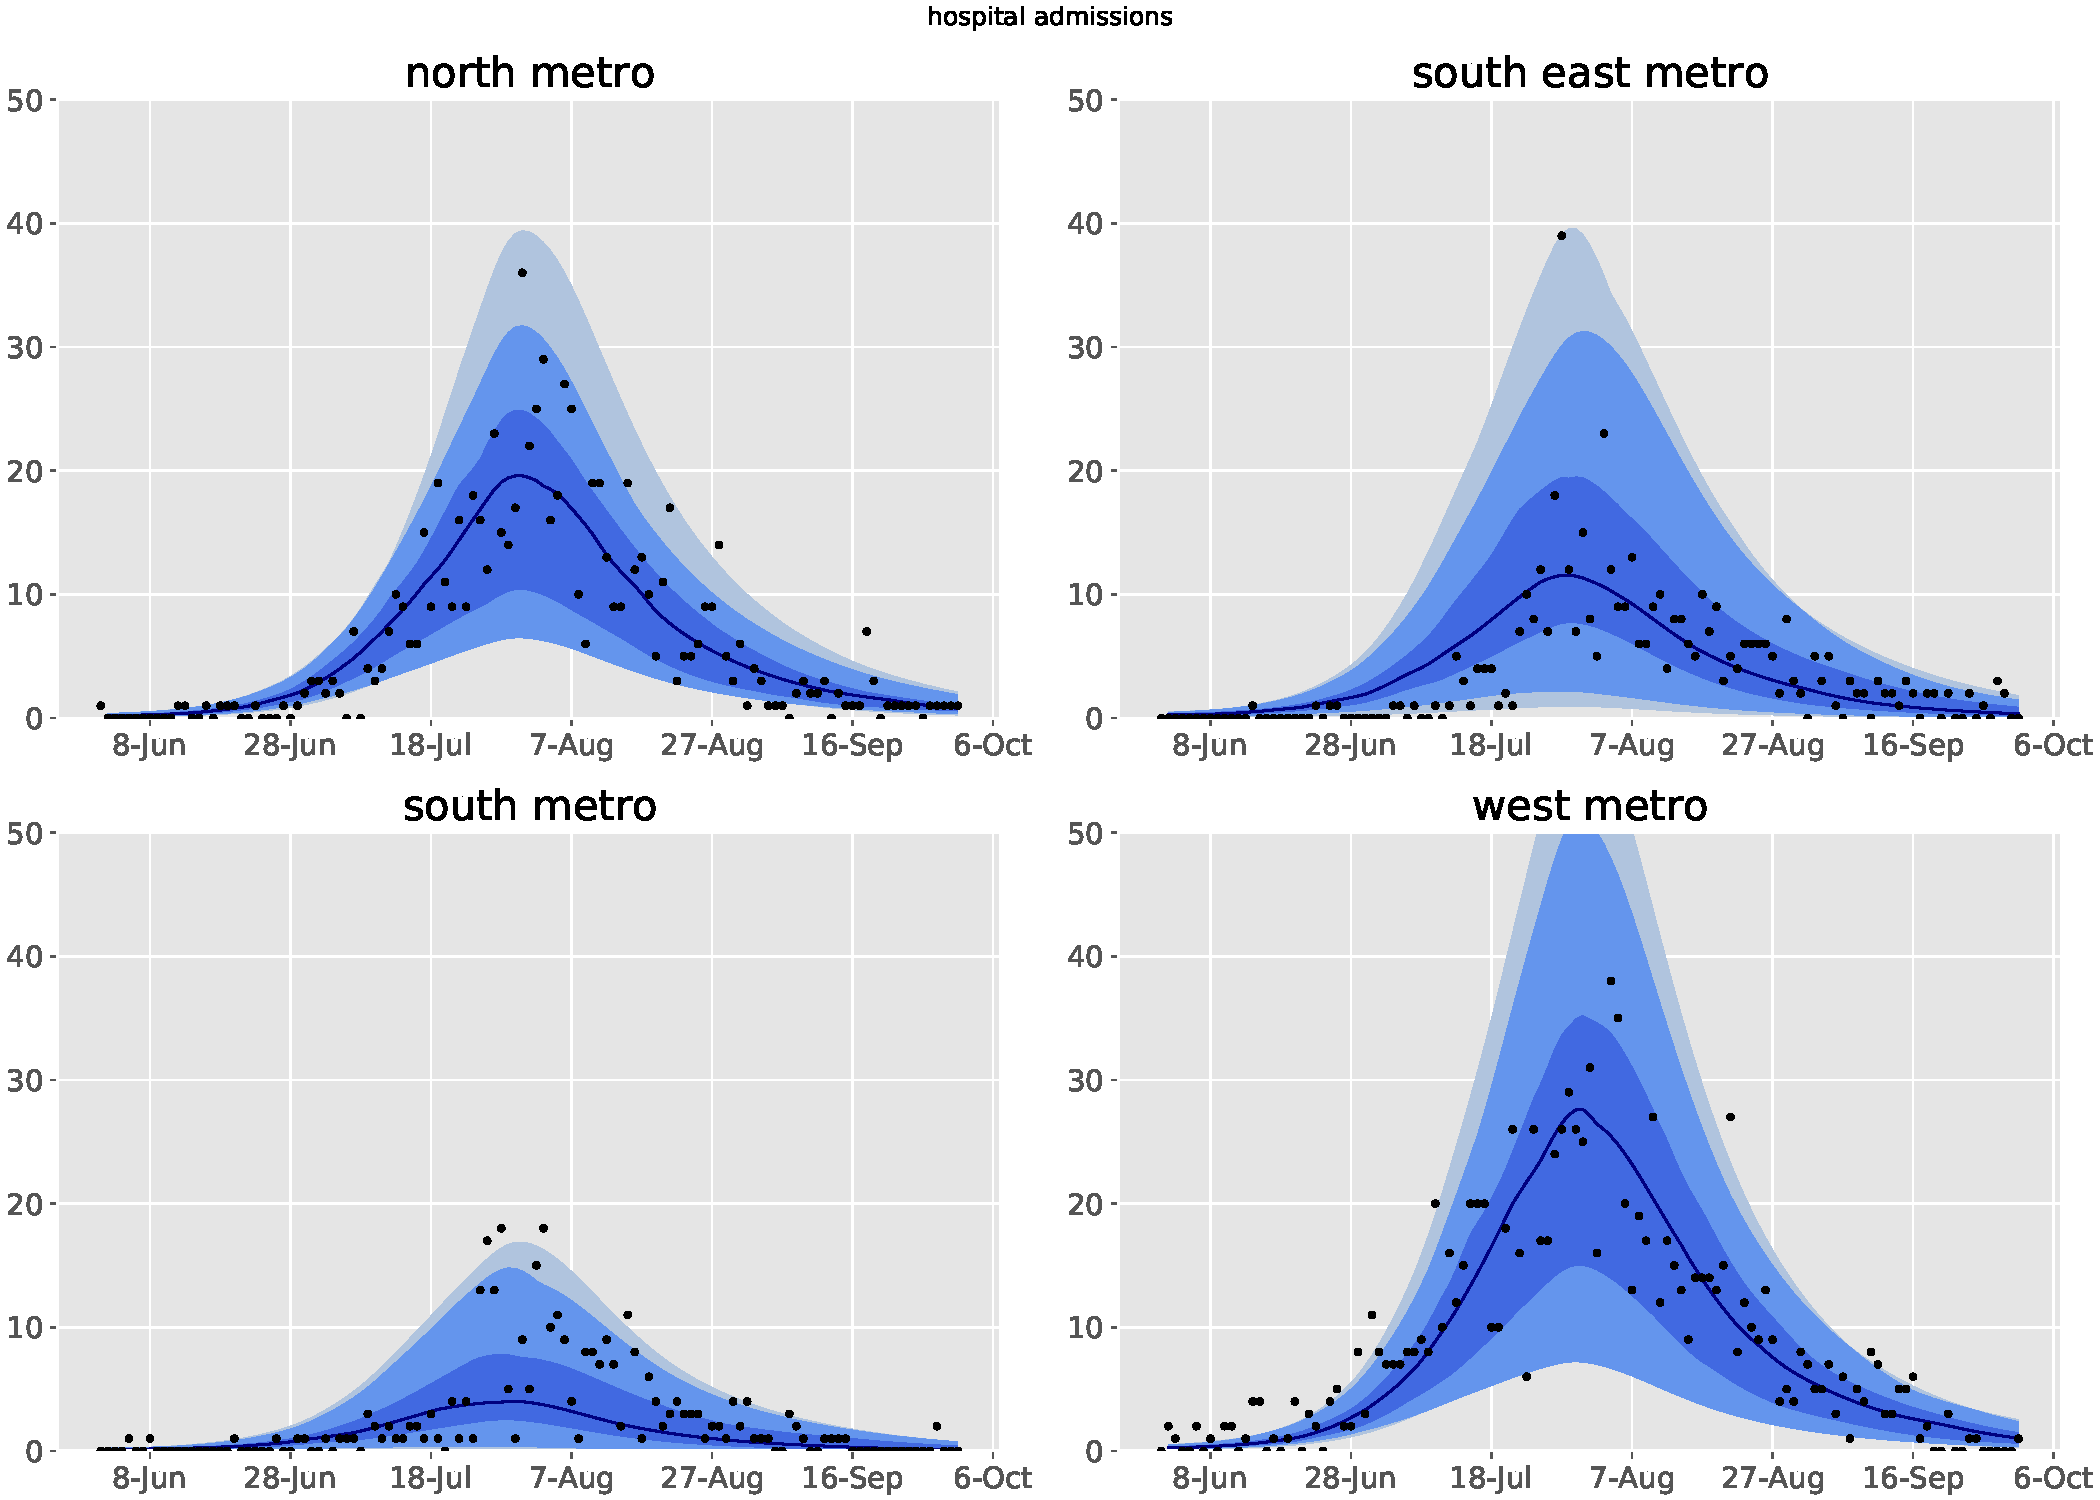
\includegraphics[scale=1]{../covid_19/projects/victoria/results_figures/metro_hospital.png}}
    \caption{\textbf{Validation fit to daily time series of hospitalisations for each metropolitan health service cluster.} Daily hospitalisation (black dots) overlaid on the median modelled hospitalisations (dark blue line), with shaded areas representing the 25\textsuperscript{th} to 75\textsuperscript{th} centile (mid blue), 2.5\textsuperscript{th} to 97.5\textsuperscript{th} centile (light blue) and 1\textsuperscript{st} to 99\textsuperscript{th} centile (faintest blue) of estimated hospitalisations.}
\end{figure}

\begin{figure}[ht]
    \resizebox{1\textwidth}{!}{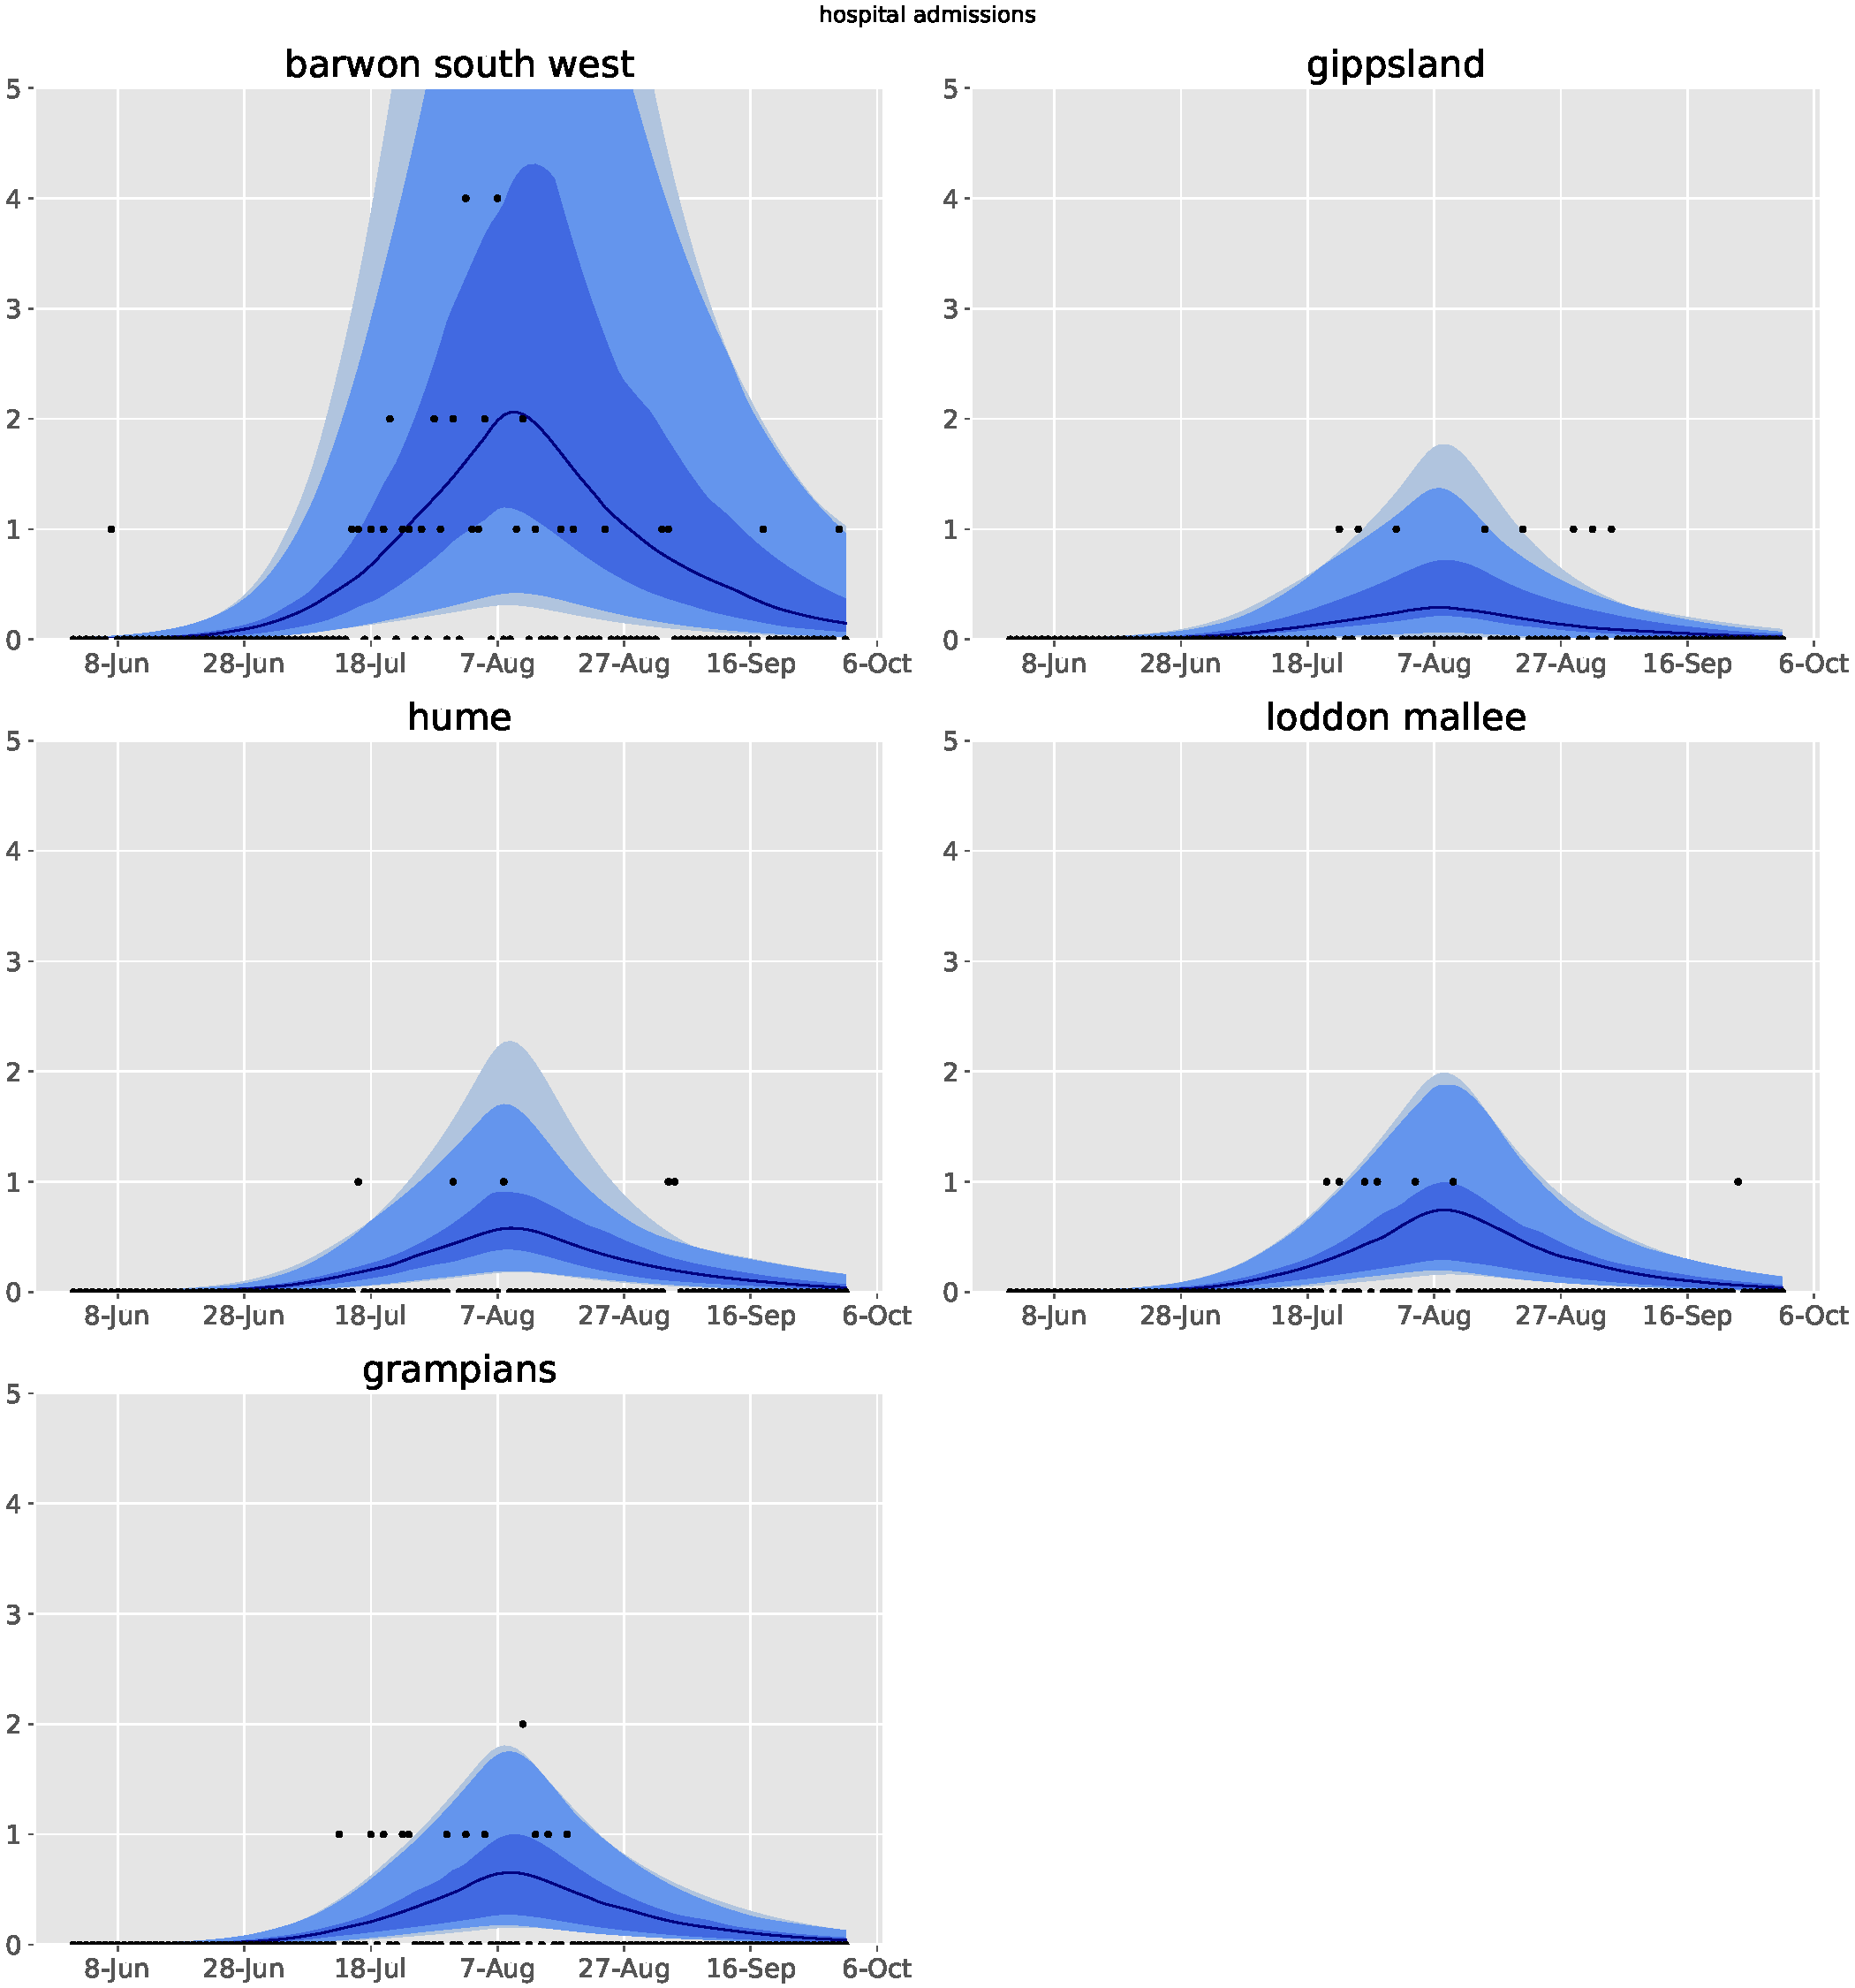
\includegraphics[scale=1]{../covid_19/projects/victoria/results_figures/regional_hospital.png}}
    \caption{\textbf{Validation fit to daily time series of hospitalisations for each regional health service cluster.} Daily hospitalisation (black dots) overlaid on the median modelled hospitalisations (dark blue line), with shaded areas representing the 25\textsuperscript{th} to 75\textsuperscript{th} centile (mid blue), 2.5\textsuperscript{th} to 97.5\textsuperscript{th} centile (light blue) and 1\textsuperscript{st} to 99\textsuperscript{th} centile (faintest blue) of estimated hospitalisations.}
\end{figure}

% ICU occupancy
\begin{figure}[ht]
    \resizebox{1\textwidth}{!}{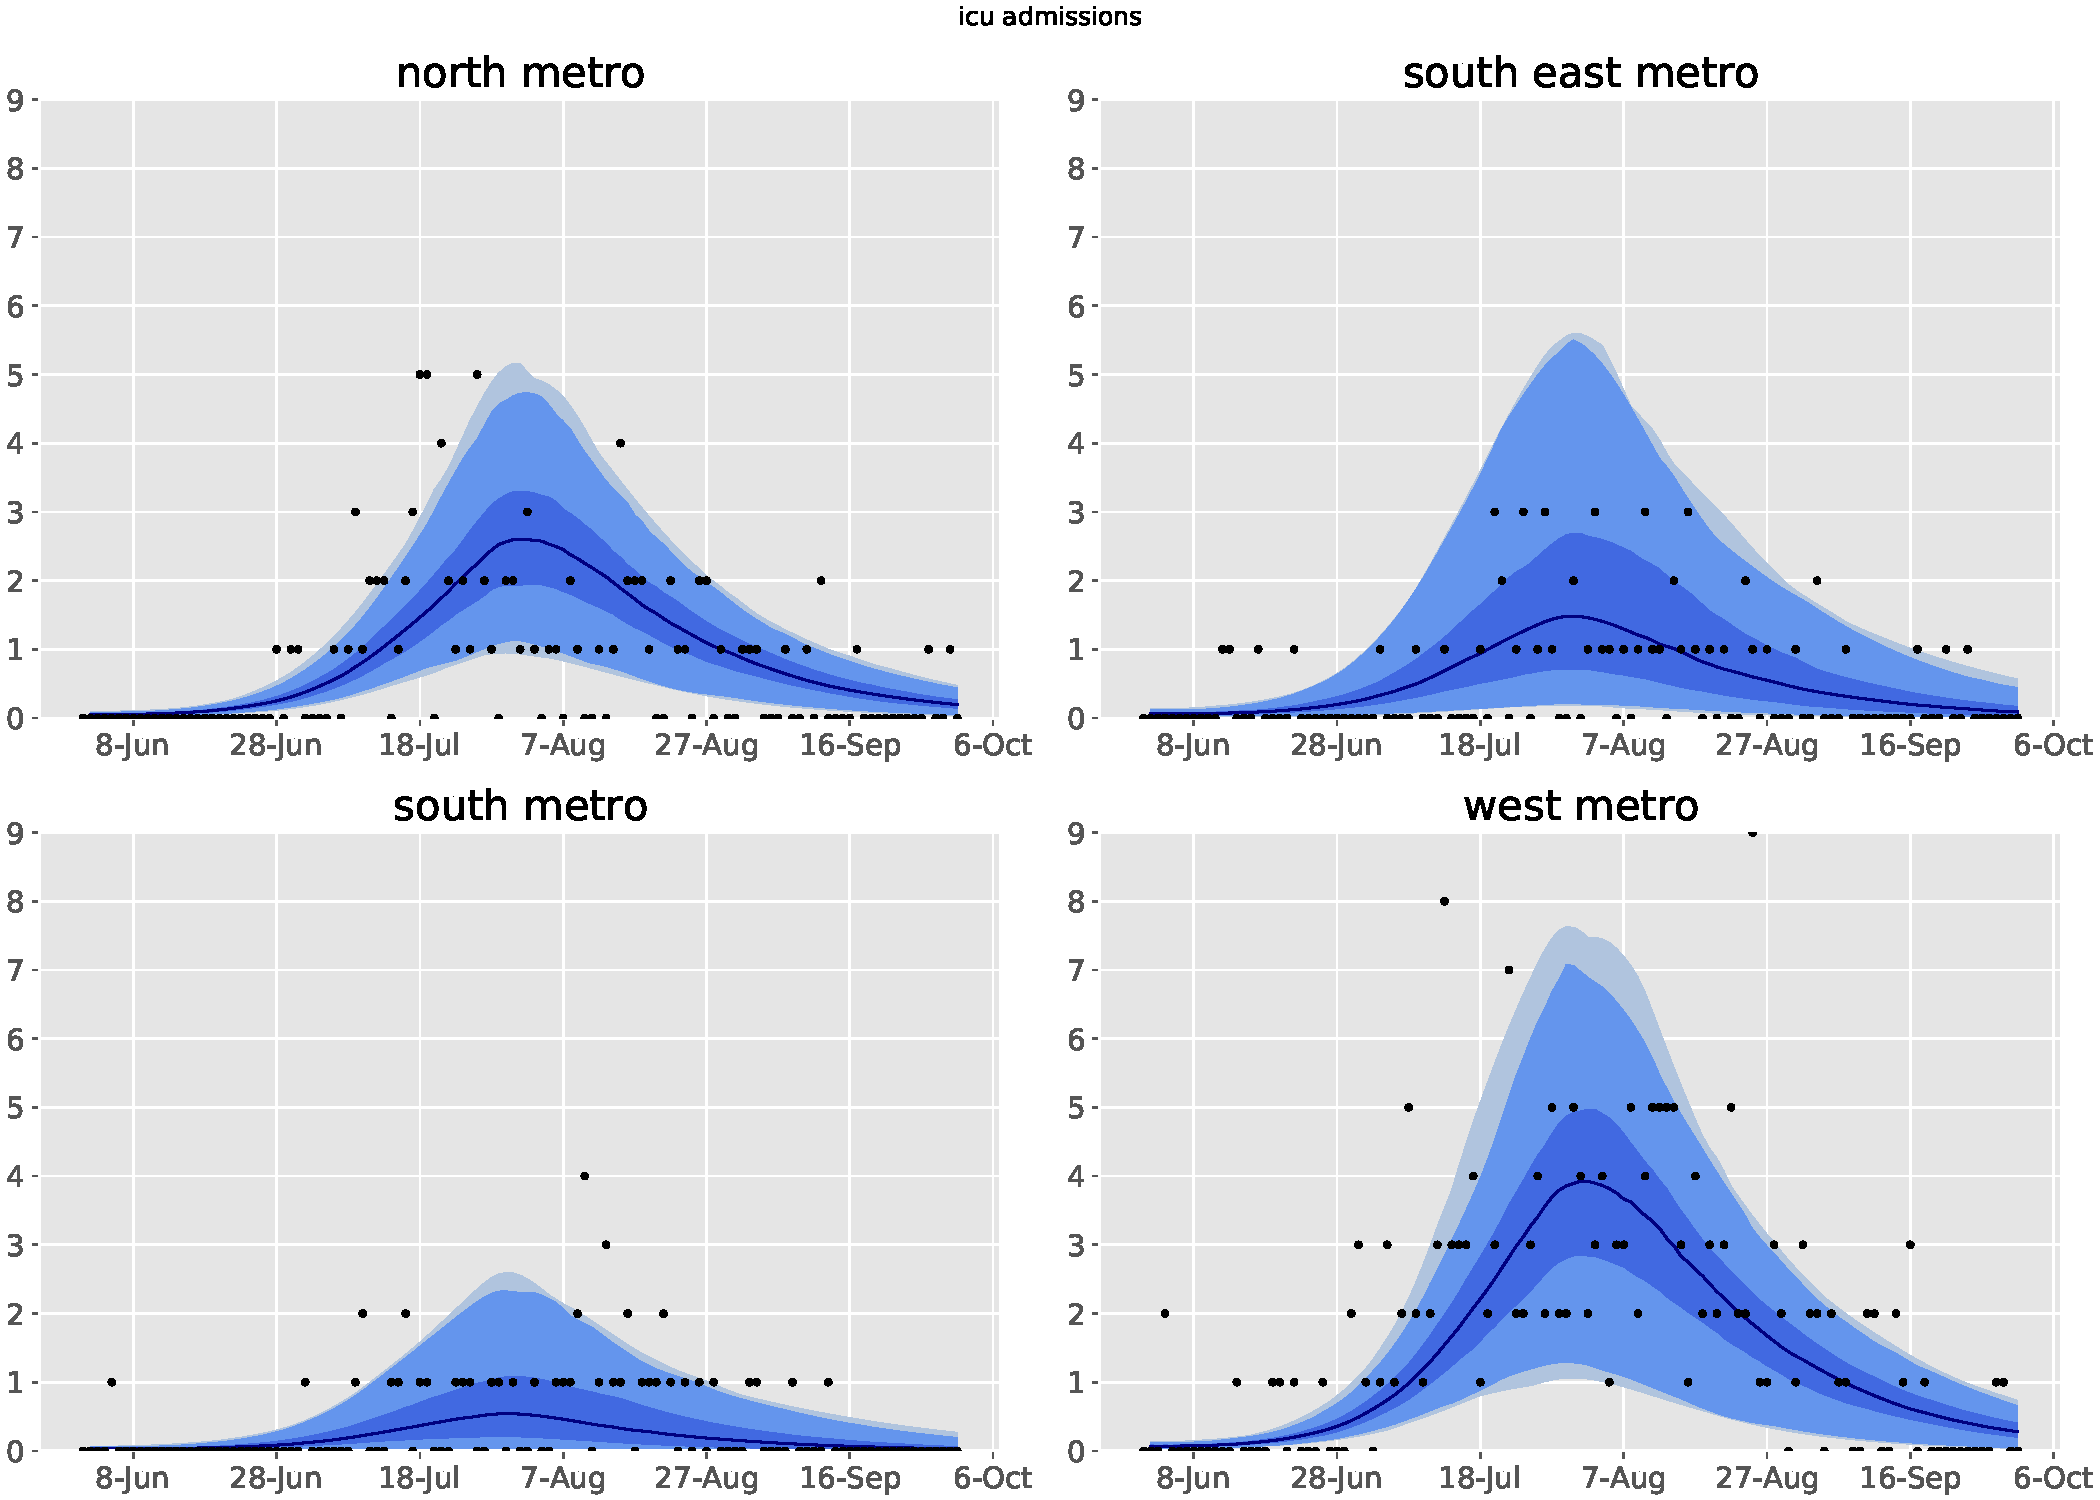
\includegraphics[scale=1]{../covid_19/projects/victoria/results_figures/metro_icu.png}}
    \caption{\textbf{Validation fit to ICU occupancy for each metropolitan health service cluster.} ICU occupancy (black dots) overlaid on the median modelled ICU occupancy (dark blue line), with shaded areas representing the 25\textsuperscript{th} to 75\textsuperscript{th} centile (mid blue), 2.5\textsuperscript{th} to 97.5\textsuperscript{th} centile (light blue) and 1\textsuperscript{st} to 99\textsuperscript{th} centile (faintest blue) of estimated ICU occupancy.}
\end{figure}

% Posterior histograms
\begin{figure}[ht]
    \resizebox{1\textwidth}{!}{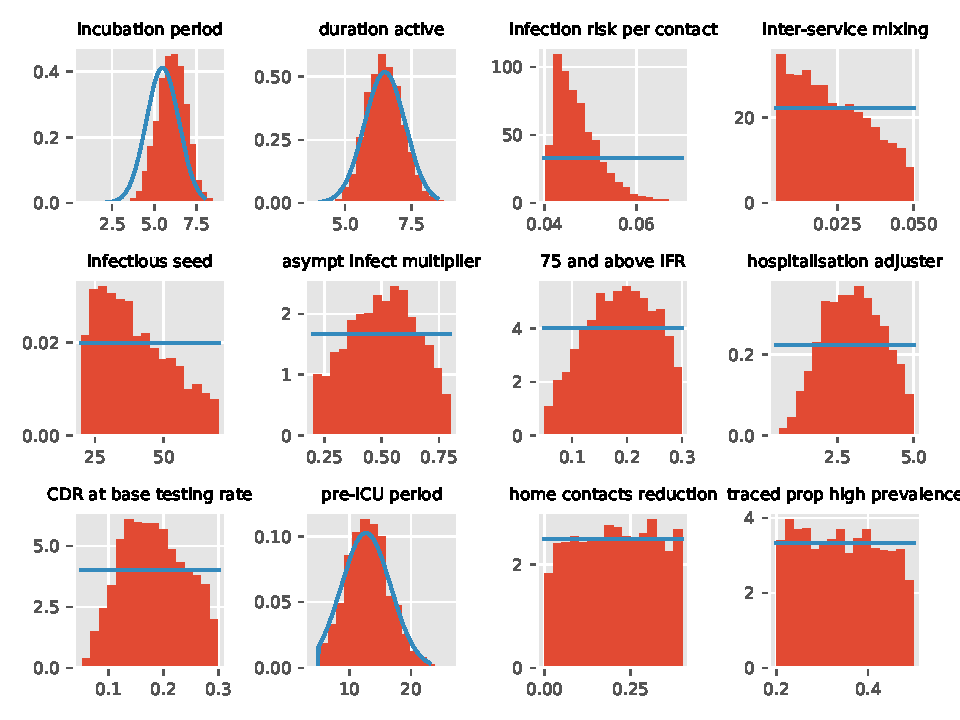
\includegraphics[scale=1]{../covid_19/projects/victoria/results_figures/epi_posteriors.png}}
    \caption{\textbf{Histograms of state-wide epidemiological parameter posteriors, other than key parameters of interest} (presented in main manuscript).}
\end{figure}

\begin{figure}[ht]
    \resizebox{1\textwidth}{!}{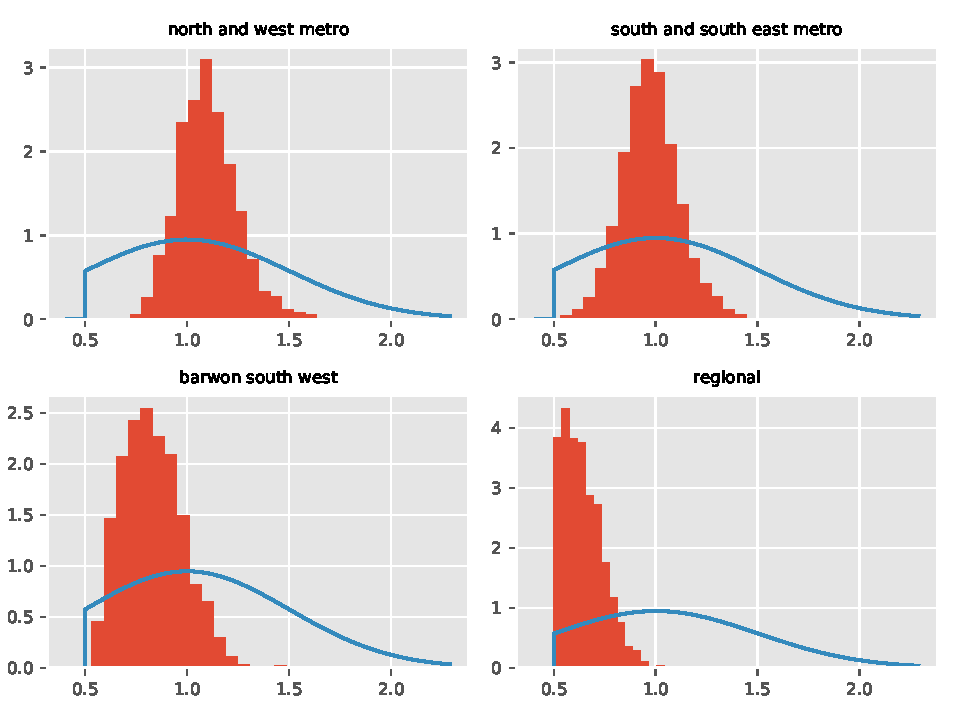
\includegraphics[scale=1]{../covid_19/projects/victoria/results_figures/contact_posteriors.png}}
    \caption{\textbf{Histograms of cluster-specific contact rate modifier parameter posteriors.}}
\end{figure}

% Parameter correlation matrices
\begin{figure}[ht]
    \resizebox{1\textwidth}{!}{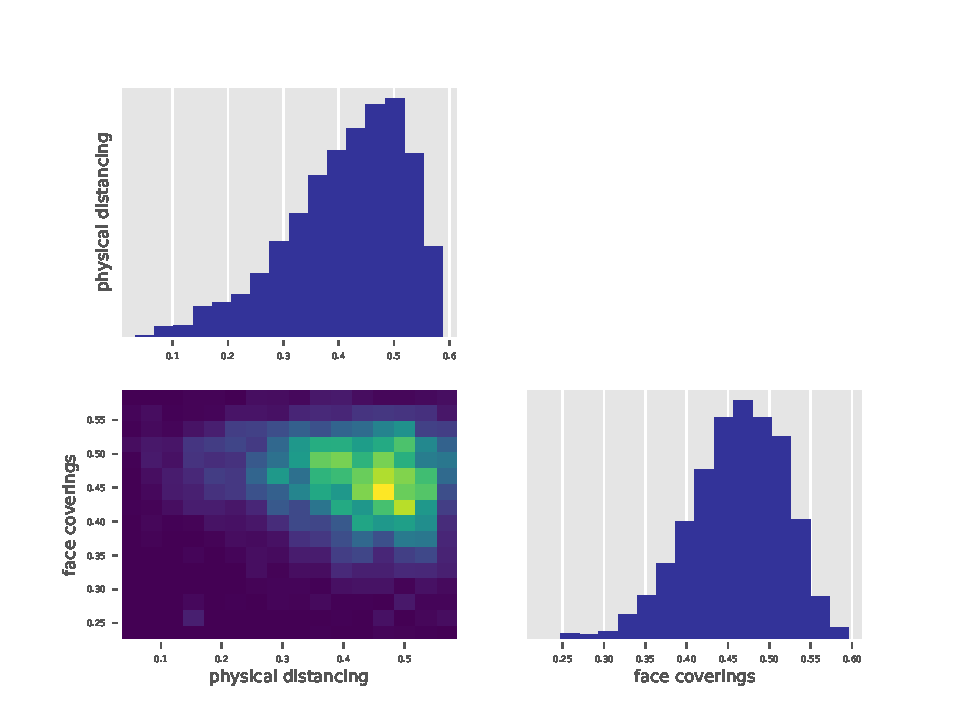
\includegraphics[scale=1]{../covid_19/projects/victoria/results_figures/key_param_matrix.png}}
    \caption{\textbf{Correlation matrix for key epidemiological parameters of interest.}}
\end{figure}

\begin{figure}[ht]
    \resizebox{1\textwidth}{!}{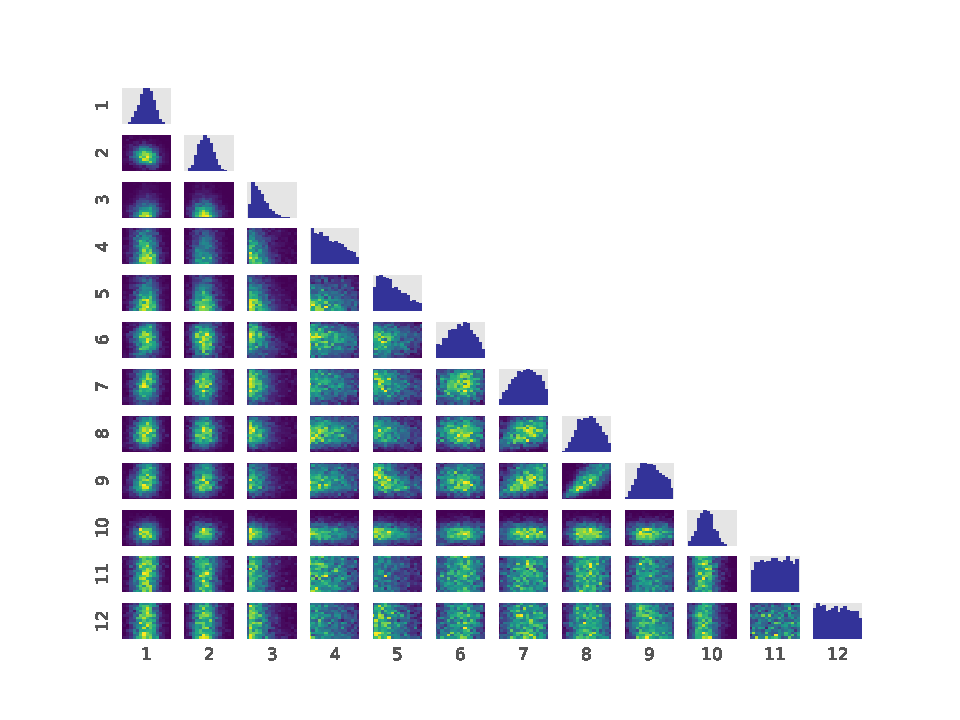
\includegraphics[scale=1]{../covid_19/projects/victoria/results_figures/epi_param_matrix.png}}
    \caption{\textbf{Correlation matrix for other state-wide epidemiological parameters.} Key: 1, incubation period; 2, duration active; 3, infection risk per contact; 4, inter-cluster mixing; 5, infectious seed; 6, sympt prop adjuster; 7, asympt infect multiplier; 8, over 75 IFR; 9, hospitalisation adjuster; 10, CDR at base testing rate; 11, pre-ICU period; 12, contact tracing assumed trace prop.}
\end{figure}

\begin{figure}[ht]
    \resizebox{1\textwidth}{!}{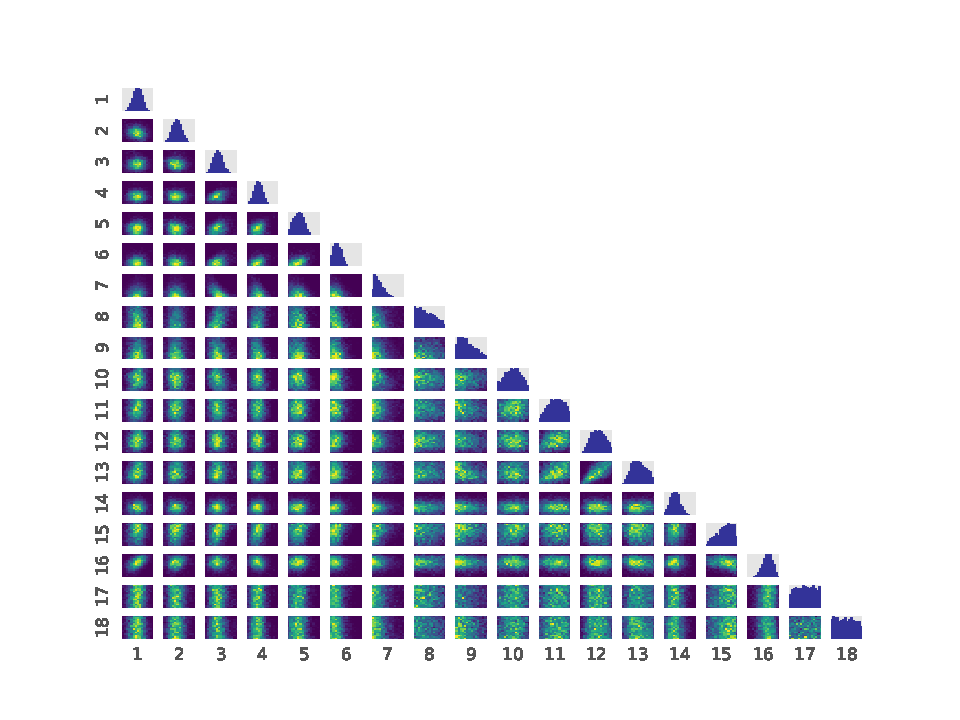
\includegraphics[scale=1]{../covid_19/projects/victoria/results_figures/all_params_matrix.png}}
    \caption{\textbf{Correlation matrix for other state-wide epidemiological parameters.} Key: 1, incubation period; 2, duration active; 3, north metro; 4, south metro; 5, barwon south west; 6, regional; 7, infection risk per contact; 8, inter-cluster mixing; 9, infectious seed; 10, sympt prop adjuster; 11, asympt infect multiplier; 12, over 75 IFR; 13, hospitalisation adjuster; 14, CDR at base testing rate; 15, pre-ICU period; 16, physical distancing; 17, face coverings; 18, target output ratio; 19, contact tracing assumed trace prop.}
\end{figure}

% Parameter traces
\begin{figure}[ht]
    \resizebox{1\textwidth}{!}{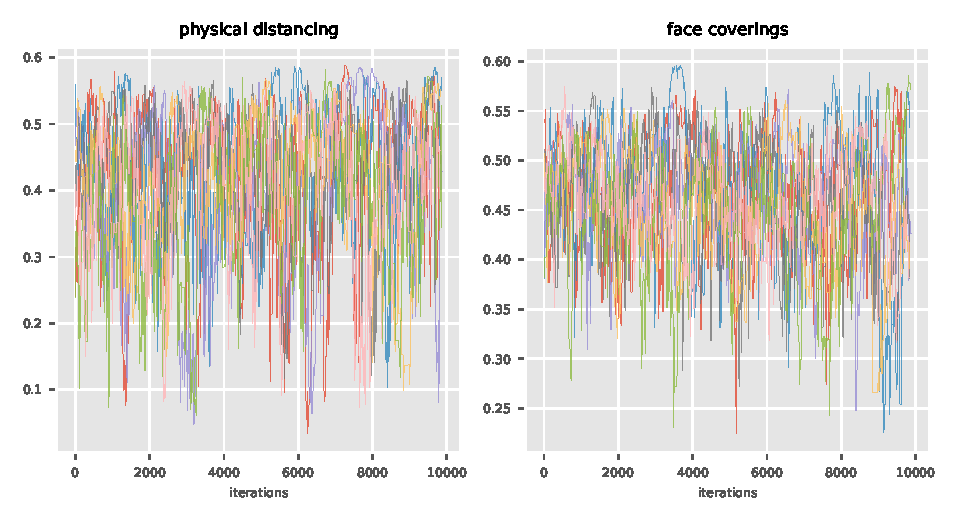
\includegraphics[scale=1]{../covid_19/projects/victoria/results_figures/key_traces.png}}
    \caption{\textbf{Parameter progression traces for key estimation parameters.}}
\end{figure}

\begin{figure}[ht]
    \resizebox{1\textwidth}{!}{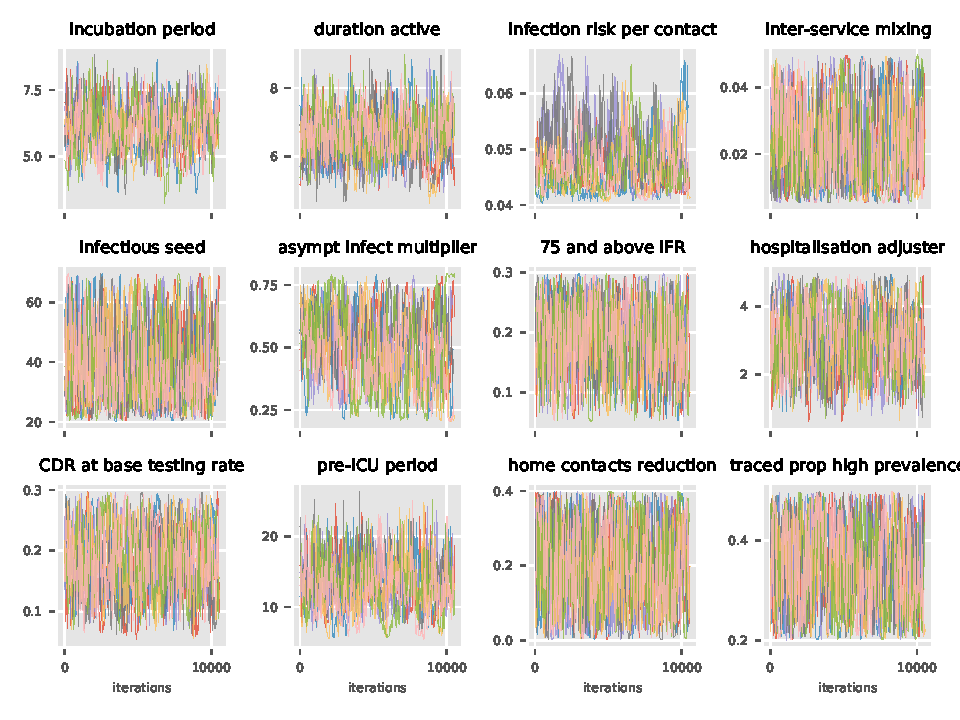
\includegraphics[scale=1]{../covid_19/projects/victoria/results_figures/epi_traces.png}}
    \caption{\textbf{Parameter progression traces for epidemiological parameters.}}
\end{figure}

\begin{figure}[ht]
    \resizebox{1\textwidth}{!}{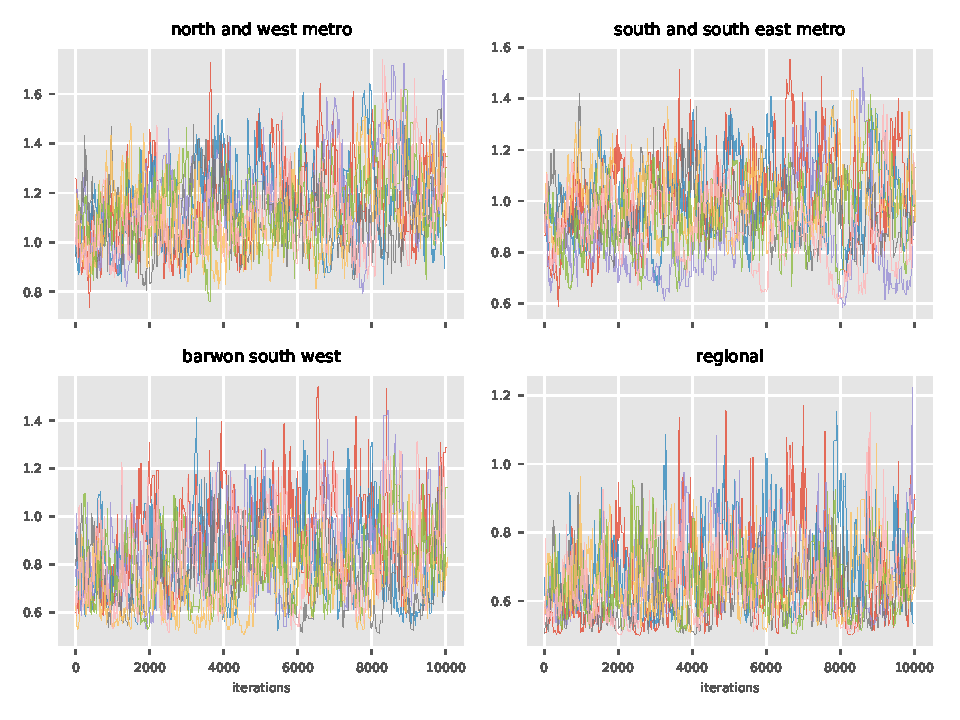
\includegraphics[scale=1]{../covid_19/projects/victoria/results_figures/contact_traces.png}}
    \caption{\textbf{Parameter progression traces for cluster contact rate modifier parameters.}}
\end{figure}

\begin{table}[ht]
\renewcommand{\baselinestretch}{1}
	\begin{tabular}[ht]{| p{7cm} | p{6cm} |}
	\hline
		\textbf{Parameter} & \textbf{Convergence statistic} (\(\hat{R}\)) \\
		
\hline incubation period & 1.081 \\

\hline duration active & 1.259 \\

\hline north and west metro & 1.191 \\

\hline south and south east metro & 1.045 \\

\hline barwon south west & 1.047 \\

\hline regional & 1.070 \\

\hline infection risk per contact & 1.653 \\

\hline inter-cluster mixing & 1.031 \\

\hline infectious seed & 1.181 \\

\hline sympt prop adjuster & 1.086 \\

\hline asympt infect multiplier & 1.636 \\

\hline 75 and above IFR & 1.081 \\

\hline hospitalisation adjuster & 1.030 \\

\hline CDR at base testing rate & 1.161 \\

\hline pre-ICU period & 1.407 \\

\hline physical distancing & 1.379 \\

\hline face coverings & 1.098 \\

\hline target output ratio & 1.038 \\

\hline contact tracing assumed trace prop & 1.134 \\

	\hline
    \end{tabular}
    \title{Chain convergence statistics.}
    \caption{\textbf{Chain convergence statistics.}}	
    \label{tab:convergence}
\end{table}


% Recovered proportion
\begin{figure}[ht]
    \resizebox{1\textwidth}{!}{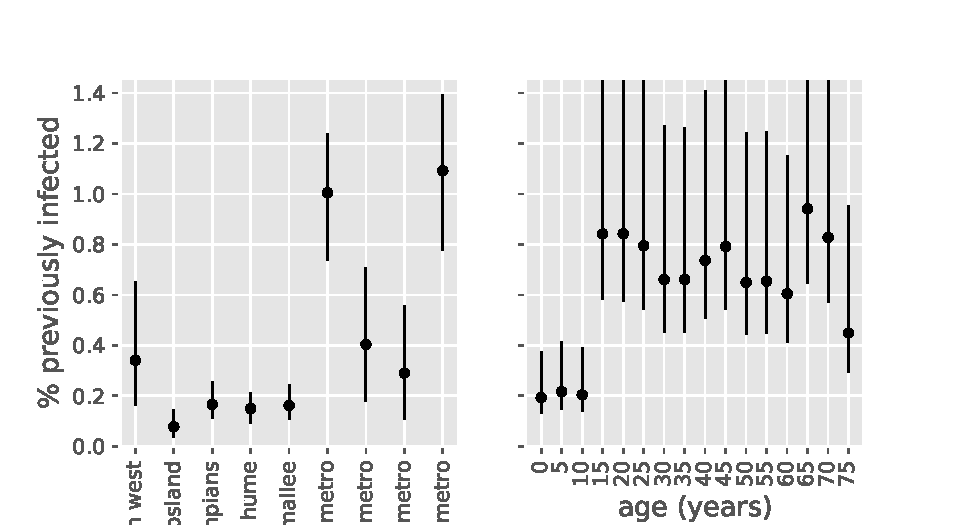
\includegraphics[scale=1]{../covid_19/projects/victoria/results_figures/sero_by_cluster.png}}
    \caption{\textbf{Estimated proportion of population recovered from COVID-19 at 1\textsuperscript{st} October 2020, by age group and health service cluster.} Point estimates with associated 50\% credible intervals. (This quantity is similar to an attack rate, except with deaths excluded from the denominator. Infections from first wave not considered.)}
\end{figure}
